\chapter{GIS.lab}
\label{2-teorie}

\begin{figure}[H] \centering
    
\includegraphics[width=80pt]{./pictures/gislab-logo.png}
    \caption[GIS.lab logo]{GIS.lab logo (zdroj:
	\href{https://github.com/gislab-npo/gislab-doc/blob/master/img/logo.svg}{GIS.lab repozitář})}
	\label{fig:gislab-logo}
\end{figure}
% zdroj: http://geo.fsv.cvut.cz/~landa/publications/2016/telc-2016/prezentace/figures/

\section{Co je to GIS.lab?}
% https://gislab.readthedocs.io/en/latest/general/about.html
% http://geo.fsv.cvut.cz/~landa/publications/2016/telc-2016/prezentace/landa-telc-2016.pdf
% http://gislab-npo.github.io/gislab/index.html

GIS.lab je nástroj pro jednoduché a rychlé nasazení (deployment)
funkční, centrálně spravované \zk{GIS} infrastruktury v jednotném
prostředí lokální sítě (\zk{LAN}), data centra nebo cloudové
služby. Jedná se o technologii, která poskytuje komplexní soubor
otevřených gisových softwarových nástrojů integrovaných do jednoho
uživatelsky přívětivého systému, jenž vyžaduje minimální náklady na
pořízení a údržbu.

\begin{figure}[H] \centering
    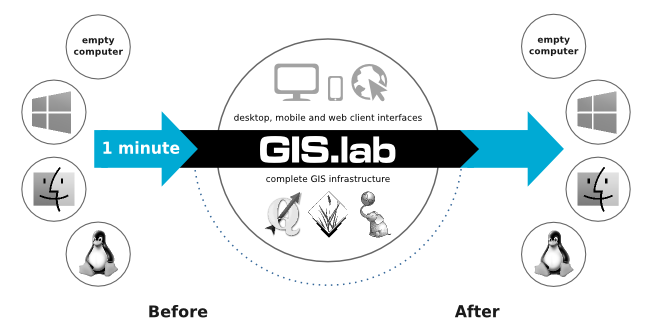
\includegraphics[width=400pt]{./pictures/gislab-schema.png}
    \caption[Schéma jednoduchosti nasazení GIS.lab]{Schéma jednoduchosti nasazení GIS.lab (zdroj:
	\href{https://github.com/gislab-npo/gislab-doc/blob/master/img/general/gislab-schema.png}{GIS.lab repozitář})}
	\label{fig:gislab-schema}
\end{figure}

K největším výhodám této platformy patří maximálně automatizovaná
instalace či rychlé nasazení pomocí GIS.lab Unit (viz
\ref{gislab-unit}), jejichž výsledkem je plně funkční a vysoce výkonný
nástroj, bez nutnosti dalšího složitého nastavení. Přizpůsobení
unikátním potřebám zákazníka je však také možné. Výpočetní kapacitu je
možné sdílet přes všechny stroje. Veškeré počítače v síti, uživatelské
účty i zálohy jsou centrálně spravované.

Z hlediska funkcionalit jsou nejzásadnější ukládání prostorově i
neprostorově orientovaných dat a jejich sdílení, tvorba a analýza
vektorových, rastrových i tabulkových dat nebo rychlé vytváření
kartografických výstupů.

Desktopový klient (tlustý klient) GIS.lab Desktop může být spuštěn v
režimu fyzickém či virtuálním. Virtuální režim lze využít na
kterémkoliv operačním systému (\zk{OS}) s tím, že původní \zk{OS} i
GIS.lab jsou přístupné. Fyzický režim umožňuje lepší výkon, který je
vykoupen dočasnou nedostupností původního \zk{OS}.

\begin{figure}[H] \centering
    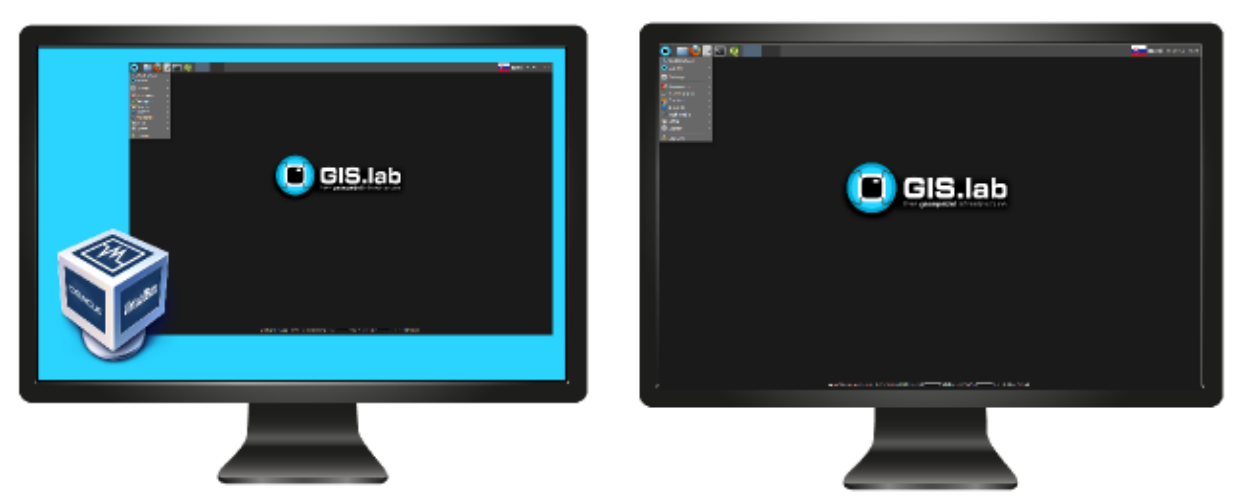
\includegraphics[width=450pt]{./pictures/physical-or-virtual-mode.png}
    \caption[Virtuální a fyzický režim GIS.lab Desktop]{Virtuální a fyzický režim GIS.lab Desktop (zdroj:
	\href{https://github.com/gislab-npo/gislab-doc/blob/master/img/installation/physical-or-virtual-mode.png}{GIS.lab repozitář})}
	\label{fig:gislab-rezim}
\end{figure}

Tlustý klient poskytuje desktopové prostředí bez zádrhelů, které se
mohou vyskytovat u tenkého klienta. Jeho využití však není primárně
zamýšleno v tradičním pojetí desktopu jako jediného klienta, ale spíše
jako jakési specializované klientské rozhraní poskytující nástroje ze
světa desktopu.

Konfiguraci a nasazení GIS.labu řídí platforma Ansible, nasazení ve
virtuálním režimu umožňuje Vagrant a VirtualBox.

GIS.lab po nasazení sestává z jednoho stroje, který zastává roli
hlavního uzlu (server), a k němu připojeného množství dalších počítačů
(klientů). Pro hlavní uzel je vyžadován stroj s operačním systémem
Linux, požadavky na klientské počítače nejsou téměř žádné - nemusí
obsahovat operační systém ani pevný disk. Je však potřeba, aby všechny
počítače v síti byly připojené pomocí gigabitového síťového kabelu a
síťového přepínače (switch).

\begin{figure}[H] \centering
    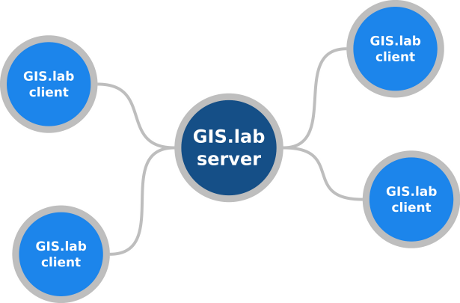
\includegraphics[width=280pt]{./pictures/gislab-architecture.png}
    \caption[GIS.lab architektura]{GIS.lab architektura (zdroj:
	\href{https://github.com/gislab-npo/gislab-doc/blob/master/img/general/gislab-architecture.png}{GIS.lab repozitář})}
	\label{fig:gislab-architecture}
\end{figure}

S pomocí integrované platformy Gisquick (viz \ref{gisquick}) podporuje
GIS.lab kromě desktopového i webového a mobilního klienta.

\subsubsection{GIS.lab unit}
\label{gislab-unit}
%http://gislab-npo.github.io/gislab/pages/gislab-unit
Zařízení s názvem GIS.lab Unit je přenosné hardwarové řešení
obsahující systém GIS.lab připravený k okamžitému zapojení a nasazení
ve zvolené síti. Jedná se o krabičku s rozměry přibližně 11 x 11 x 4
cm, procesorem Intel Haswell, SSD diskem a 16 GB RAM. Maximální
testované množství klientských počítačů je 20.

\begin{figure}[H] \centering
    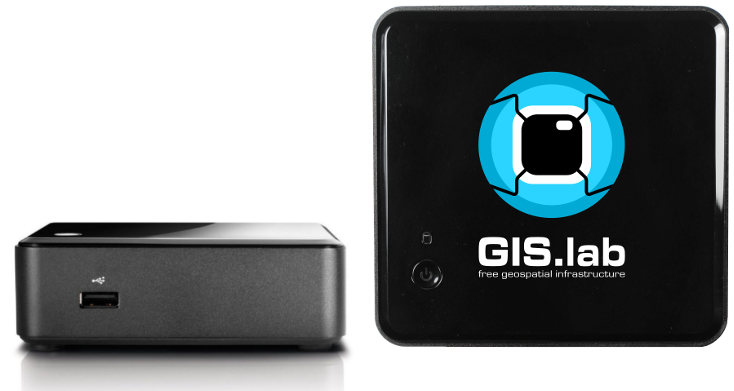
\includegraphics[width=350pt]{./pictures/gislab-unit.png}
    \caption[GIS.lab Unit]{GIS.lab Unit (zdroj:
	\href{https://github.com/gislab-npo/gislab-doc/blob/master/img/general/gislab-unit.svg}{GIS.lab repozitář})}
    \label{fig:gislab-unit}
\end{figure}

GIS.lab Server běží na operačním systému Linux, nasazení spravuje
platforma Ansible a k ověření a správě uživatelů využívá protokol
LDAP, přesněji jeho nadstavbu OpenLDAP. Software dostupný po instalaci
pro uživatele GIS.lab Desktop je uveden v následujícím seznamu:
\begin{itemize}
\item Operating system: Ubuntu Linux LTS
\item Desktop environment: XFCE
\item Office suite: LibreOffice
\item Web browser: Firefox
\item Graphics editor: GIMP, Inkscape
\item Video player: VLC
\item Secure data storage: KeepassX
\item Database management: PgAdmin, SpatiaLite GUI
\item GIS software: QGIS, GRASS GIS
\item Virtual client support: VirtualBox Guest Additions
\end{itemize}

\section{Gisquick}
\label{gisquick}
% http://gisquick.org - využila jsem 
% https://gisquick.readthedocs.io/en/latest/user-manual/project-publishing.html - nevyužila jsem 

\begin{figure}[H] \centering
    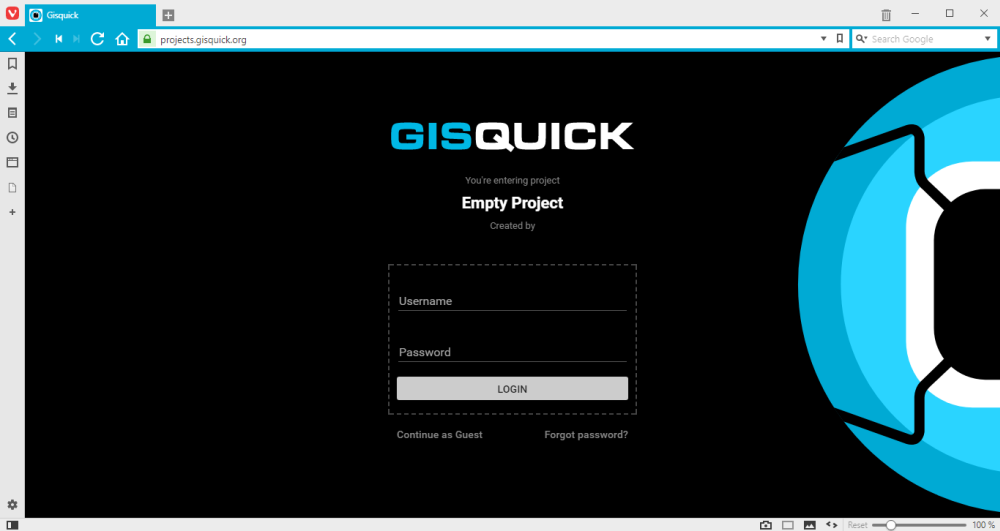
\includegraphics[width=400pt]{./pictures/gisquick-welcome-screen.png}
    \caption[Gisquick - přihlašovací stránka]{Gisquick - přihlašovací stránka (zdroj:
	\href{}{Tereza Kulovaná})}
    \label{fig:gisquick-welcome}
\end{figure}

Gisquick je open-source platforma umožňující publikaci geoprostorových
dat. Byla vytvořena s cílem snadného sdílení projektů vytvořených v
desktopové aplikaci QGIS na webu. Gisquick sestává ze zásuvného modulu
QGIS, QGIS serveru, serverové aplikace založené na frameworku Django,
webového a mobilního klienta. Obsahuje základní sadu nástrojů
potřebných pro webovou mapovou aplikaci. Plně responzivní uživatelské
rozhraní (\zk{UI}) je optimalizováno i pro mobilní zařízení.

Gisquick byl vyvíjen jako součást GIS.labu, ale v roce 2015 se oddělil
jako samostatný projekt. Dnes je možné ho tedy využívat samostatně,
zároveň však zůstává integrován v každé instalaci GIS.labu a rozšiřuje
jeho funkcionalitu.

Je distribuován pod otevřenou licencí GNU \zk{GPL} v2.0.

\section{Aktuální využití}
\label{gislab-vyuziti}

V současné době se GIS.lab využívá především při výuce na Fakultě
stavební ČVUT v rámci hodin zaměřených na \zk{GIS} a dálkový průzkum
Země (\zk{DPZ}). Také na něm probíhají některá školení skupiny
Gismentors.

Vyučování probíhá ve fyzickém režimu GIS.lab Desktop s nasazením
pomocí GIS.lab Unit. Každý student má vytvořen vlastní uživatelský
účet a dedikované schéma v databázi. Studenti jsou seznámeni s
připojením k databázi pomocí PgAdmin, většinou je však využíváno
připojení přes QGIS. QGIS je také upřednostňovaným softwarem při
zpracování prostorových i neprostorových dat, výhodou je i možnost
využívat zásuvný modul Gisquick pro publikaci dat v podobě webových
aplikací. Přesto jsou studenti krátce seznámeni s programem GRASS GIS,
strukturou GRASS projektů a práce s nimi. GRASS GIS je více využíván v
rámci předmětů orientovaných na \zk{DPZ}, jelikož obsahuje dobře
implementované nástroje pro zpracování obrazových dat. K nástrojům
GRASS GIS mohou uživatelé přistupovat i přes QGIS \zk{UI} díky
předinstalovanému zásuvnému modulu QGIS GRASS.

Komunikace probíhá přes zabudovanou IRC službu, kterou lze využít mimo
jiné pro okamžité a jednoduché sdílení nezbytných příkazů či
potřebných webových adres. Pro sdílení souborů jsou určené dvě složky,
k nimž mají přístup všichni připojení uživatelé. Pro standardní výměnu
mezi klientskými počítači je příhodnější složka \textit{Barrel} s
právy čtení i zápisu pro všechny. Data trvalejšího charakteru je
vhodné umístit do adresáře \textit{Repository}, odkud je možné data
stahovat, ale upravovat je mohou pouze správci.

\section{Plány na rozšíření}
\label{vision}

Autoři GIS.labu by rádi v budoucnu rozšířili uživatelskou základnu,
proto mají za cíl práci správcům i uživatelům zpříjemnit a nabídnout
co nejširší portfolio služeb.

\begin{figure}[H] \centering
    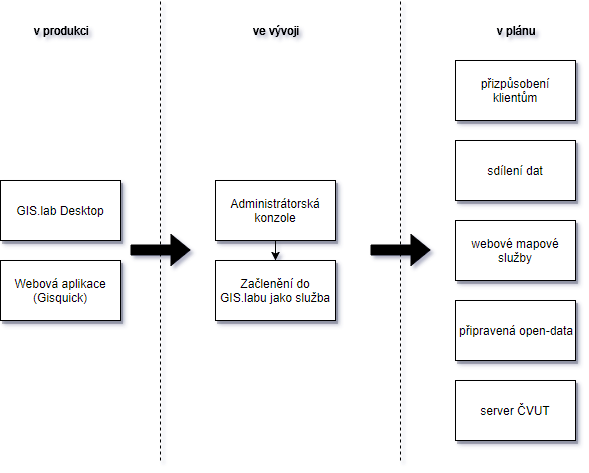
\includegraphics[width=350pt]{./pictures/gislab_road_map.png}
    \caption[Vývoj GIS.labu]{Vývoj GIS.labu (zdroj:
	\href{}{Tereza Kulovaná})}
    \label{fig:gislab-roadmap}
\end{figure}

\subsubsection{přizpůsobení klientským požadavkům}
První plánovanou změnou je umožnit zákazníkům přizpůsobit platformu
GIS.lab konkrétním požadavkům již při nasazení pomocí Ansible
playbooks (viz \ref{docker}), které se vyznačují pro člověka snadno
čitelným jazykem. Aktuálně jsou již využívány pro plně automatizovanou
instalaci, zatímco chování systému během vytváření a odstraňování
uživatelských účtů je definováno v pěti speciálních skriptech, psaných
v bashi:
\begin{itemize}
\item \texttt{before-add} - spuštěn před vytvořením účtu
\item \texttt{after-add} - spuštěn po vytvoření účtu
\item \texttt{before-delete} - spuštěn před odstraněním účtu
\item \texttt{after-delete} - spuštěn po odstranění účtu
\item \texttt{files} - obsah tohoto adresáře je zkopírován do domovského adresáře uživatele předtím než je spuštěn skript \texttt{after-add}
\end{itemize}
Příkladem využití skriptu \texttt{after-add} by se v případě databáze
mohlo například týkat volby jakým způsobem umožnit uživateli přístup k
databázi, zda mu vytvořit vlastní nebo jen schéma v již
existující. Následně je třeba také vyřešit, zda při odstranění účtu
dojde pouze ke smazání dat nebo zda z nich vytvořit tzv. dump, který
uživateli zaslat.

Právě obsah těchto skriptů by mohl být také definován v Ansible
playbooks. Ukázky nejvyužívanějších nastavení budou dostupné v Github
repozitáři.

\subsubsection{sdílení dat}

V případě fyzického režimu GIS.lab Desktop jsou veškerá vytvořená data
dostupná pouze v rámci klienta, na němž GIS.lab běží, sdílet s dalšími
uživateli je lze pouze přes společné adresáře \textit{Repository} a
\textit{Barrel} nebo v případě publikace jako mapové aplikace skrz
Gisquick. V případě adresářů jsou data přístupná všem uživatelům v
rámci sítě bez rozdílu, u mapové aplikace každému se správnou webovou
adresou.
% je to pravda? jak jsou vlastně přístupné aplikace přes gisquick?

Pokud by se chtěl uživatel podělit o přístup k některé části své
databáze, bude k tomu moci v první fázi využít SQL příkazu GRANT,
později pak vyhledat jiného uživatele přes webovou administrátorskou
konzoli a přístup mu udělit přes ni.

Pokud má uživatel zájem data přenést z klienta pryč nebo naopak nějaká
data nahrát, musí k tomu využít mezistupeň v podobě externího disku,
ať už reálného či virtuálního. Ideální by proto byla možnost
přistupovat vzdáleně nejen k databázi, ale například i k oddílu na
serveru obsahujícím data ve formátu Esri Shapefile (.shp) či
GeoPackage (.gpkg). Tuto variantu bude umožňovat sdílení pomocí služby
NFS (Network File System). Tímto způsobem budou moci uživatelé
pracovat s daty i při běhu svého standardního \zk{OS}.

\subsubsection{webové mapové služby}

Publikaci dat mimo síť GIS.lab umožňuje integrovaná služba Gisquick, s
jejíž pomocí lze vytvářet webové mapové aplikace. Někteří uživatelé by
však zajisté rádi publikace WMS, WFS služeb, publikace přes Gisqsuick

\subsubsection{připravená open-data}

Část dat už je v rámci státní správy České republiky poskytovaná ve
formě otevřených dat. Ne všichni zájemci o ně však vědí, kde zmiňovaná
data najít, případně jak je dostat do formátu vhodného k dalším
analýzám. Právě pro ně bude vhodná další služba.

Pokud si správce zvolí, GIS.lab server bude obsahovat stažená
geoprostorová data, především z Českého úřadu zeměměřického a
katastrálního (ČÚZK) - územní jednotky, Registr územní identifikace,
adres a nemovitostí (RÚIAN), apod. Na datové sady budou po stažení
aplikovány testy datové integrity, případné nekonzistence budou
odstraněny a výsledek bude začleněn do PostGIS databáze.

Konkrétní datové sady a tempo jejich aktualizací bude rozhodnuto až
při reálné implementaci.

\subsubsection{server ČVUT}
Snaha o rozšíření základny uživatelů platformy GIS.lab cílí v
nejbližší době především na studenty ČVUT a to i mimo Fakultu
stavební. V prvním kroku již byly získány prostředky, jež umožňují
spuštění GIS.lab přes server ČVUT. Pro jednotlivé fakulty či katedry,
které by se jej rozhodly využívat, bude připraveno několik základních
přizpůsobení, hlavně s ohledem na datové sady z veřejného sektoru.

\subsubsection{webová administrátorská konzole}

Nejblíže zařazení na seznam služeb je webové rozhraní pro správu
uživatelů, které je zpracováváno v rámci této diplomové
práce. Aktuálně používaný systém správy uživatelů je funguje na bázi
příkazové řádky a je popsán v kapitole \ref{cmd-line}.




\begin{figure}[H] \centering
    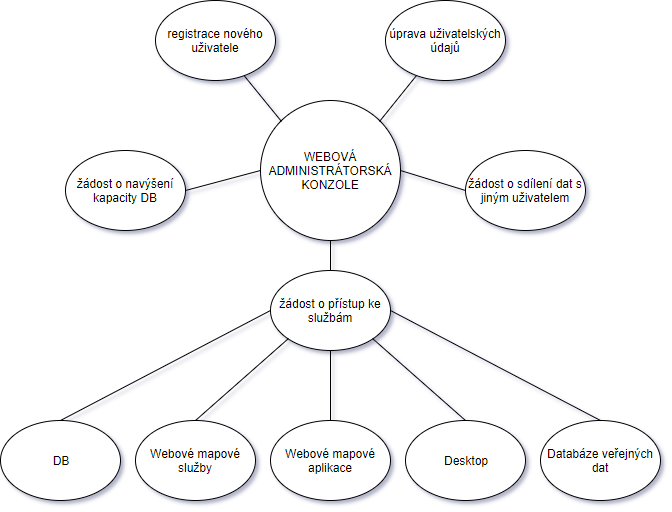
\includegraphics[width=350pt]{./pictures/console_services.png}
    \caption[Služby poskytované webovou administrátorskou konzolí]{Služby poskytované webovou administrátorskou konzolí (zdroj:
	\href{}{Tereza Kulovaná})}
    \label{fig:konzole-sluzby}
\end{figure}
